\swjtuChapter{软件需求规格说明书}

% 去掉章节前缀，使用 1 / 1.1 / 1.1.1 的编号体系
\setcounter{section}{0}
\renewcommand{\thesection}{\arabic{section}}
\renewcommand{\thesubsection}{\thesection.\arabic{subsection}}
\renewcommand{\thesubsubsection}{\thesubsection.\arabic{subsubsection}}

\section{概述}

\subsection{背景}
随着人工智能（AI）与计算机视觉（CV）技术的飞速发展，传统零售行业的数字化转型已成为必然趋势。传统商超主要依赖人工盘点与条码扫描结算，存在结算高峰期拥堵、用户寻物困难、库存数据更新滞后等显著痛点。本项目旨在利用先进的深度学习目标检测算法，结合 Web 全栈技术，开发一套低成本、高效率的“零售物品智能识别系统”，以期实现商超场景下的视觉导购、无感自助结算及供应链自动预警，全面提升运营效率与顾客体验。

\subsection{编写目标}
本文档旨在全面、准确地描述“零售物品智能识别系统”的功能性需求与非功能性需求。本文档将作为项目架构设计、代码编码、软件测试以及最终期末验收的核心基准文件，确保开发人员、测试人员与系统干系人对系统边界和业务逻辑达成一致理解。

\subsection{相关术语定义}
\begin{itemize}[leftmargin=2em]
  \item CV (Computer Vision)：计算机视觉，一门研究如何使机器“看”的科学，本系统中主要用于处理摄像头视频流。
  \item YOLO (You Only Look Once)：一种端到端的实时目标检测（Object Detection）算法，本系统采用其轻量级版本实现商品的毫秒级定位与分类。
  \item B/S 架构（Browser/Server）：浏览器/服务器模式，本系统的主要网络架构，用户只需通过浏览器即可访问系统，无需安装客户端。
  \item FastAPI：一个现代、快速（高性能）的 Python Web 框架，基于标准 Python 类型提示，用于构建本系统的后端 API 接口。
  \item ORM (Object-Relational Mapping)：对象关系映射，本系统通过 SQLAlchemy 实现面向对象的数据库操作，避免直接拼接 SQL 语句引发的安全风险。
\end{itemize}

\subsection{参考资料}
\begin{enumerate}[leftmargin=2em]
  \item 《软件工程：实践者的研究方法》
  \item YOLO 官方技术文档与学术论文
  \item FastAPI 与 SQLite 官方开发指南
\end{enumerate}

\section{总体要求}

\subsection{现状及痛点}
\begin{itemize}[leftmargin=2em]
  \item 顾客导向不足：在大型或陌生商超中，顾客往往难以快速定位所需商品，缺乏有效的室内视觉导航手段。
  \item 收银效率瓶颈：传统扫码结账需人工逐一寻找条形码，效率低下，高峰期极易造成排队拥堵。
  \item 库存管理滞后：依赖人工周期性盘点，无法做到数据的实时同步；缺货往往在顾客反馈后才被发现，导致销售机会流失。
\end{itemize}

\subsection{系统目标}
构建一个集“智能寻物、快捷收银、自动化库存管理”于一体的闭环平台。核心目标包括：
\begin{enumerate}[leftmargin=2em]
  \item 实现毫秒级的商品视觉定位与识别。
  \item 提供流畅的前后端交互，实现一键式购物车结算。
  \item 建立基于阈值的智能库存预警机制，实现供应自动化流转。
\end{enumerate}

\subsection{用户及角色分析}
\begin{itemize}[leftmargin=2em]
  \item 顾客（Customer）：核心最终用户。主要需求为浏览在售商品、通过视觉系统定位商品位置、管理购物车及完成最终支付。
  \item 商超管理员（Admin）：后台运维主体。主要需求为录入商品基础信息（名称、单价、初始库存）、处理缺货告警、查看销售统计报表。
  \item 系统定时任务（System Cron）：自动化执行代理。在后台静默运行，负责在每次交易发生后校对库存水位，并自动向虚拟供应商派发补货工单。
\end{itemize}

\subsection{系统边界及上下文环境}
\begin{itemize}[leftmargin=2em]
  \item 系统内边界：包含基于 HTML/JS 的前端交互界面、基于 Python FastAPI 的业务逻辑控制层、基于 YOLO 的视觉推理子进程、以及 SQLite 关系型数据库。
  \item 系统外边界：物理图像输入设备（USB 摄像头或监控探头）、操作系统的底层文件系统（用于存储模型权重）、模拟的第三方支付网关。
\end{itemize}

\section{功能性需求}

\subsection{主业务流程分析}

\subsubsection{核心导购与结算业务分析（UC-01）}
本业务流程涵盖了用户从进入系统到完成闭环的完整生命周期。

\begin{itemize}[leftmargin=2em]
  \item 业务描述：
\end{itemize}
\begin{enumerate}[leftmargin=2.6em]
  \item 用户进入系统并验证身份。
  \item 用户浏览商品列表，可选择直接加入购物车，或触发“视觉定位”请求。
  \item 若触发定位，系统唤起本地摄像头子进程，利用 AI 算法在视频流中实时高亮目标商品（绘制 Bounding Box 与中心坐标）。
  \item 用户将所需商品全部加入购物车后发起结算。系统校验库存充足性，计算总价并生成订单。
  \item 结算成功后，系统并行触发库存核查机制；若库存低于设定阈值，则自动执行补货逻辑。
\end{enumerate}

\begin{itemize}[leftmargin=2em]
  \item 角色参与说明：
  \item 顾客：业务的发起者与主要操作者，负责下达定位指令、确认购物车清单并支付。
  \item AI 视觉模块：作为硬件交互执行者，响应顾客请求，提供毫秒级的商品视觉坐标。
  \item 后端系统（FastAPI + SQLite）：作为业务大脑，负责拦截非法请求、执行库存扣减的原子操作，并判断是否触发下游链路。
\end{itemize}

\begin{center}
  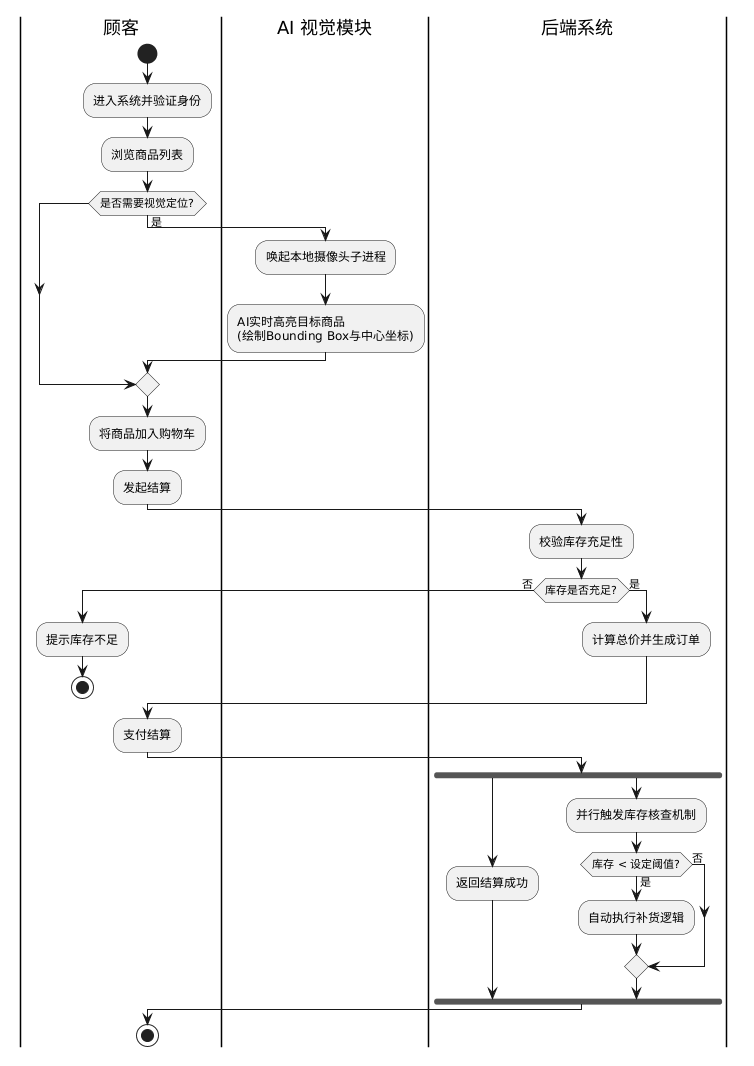
\includegraphics[width=0.88\textwidth]{images/图3-1.png}\\[0.3em]
  {\zihao{-5}图3-1}
\end{center}

\subsubsection{商品上架与基础数据维护业务分析（UC-04）}
本业务流程主要描述商超管理员如何对系统底层的商品字典和库存容量进行初始化及日常维护。

\begin{itemize}[leftmargin=2em]
  \item 业务描述：
\end{itemize}
\begin{enumerate}[leftmargin=2.6em]
  \item 商超管理员登录系统后台管理面板。
  \item 选择“商品录入/更新”功能模块。
  \item 输入商品的英文标识（需严格匹配 YOLO 模型的 names 标签）、零售单价以及入库数量。
  \item 后端系统接收到数据后，对数据库进行 Upsert（更新或插入）防重载校验。
  \item 如果数据库中已存在该商品，则将新入库数量与原有库存进行累加，并以最新填报的价格覆盖旧价格。
  \item 如果是全新商品，则在数据库中插入一条全新记录。
\end{enumerate}

\begin{itemize}[leftmargin=2em]
  \item 角色参与说明：
  \item 商超管理员：数据的提供者，确保录入的商品标识与 AI 视觉模型训练集分类保持强一致性。
  \item 后端系统：数据校验者，保证商品数据的唯一性，防止因重复录入导致数据库出现脏数据。
\end{itemize}

\begin{center}
  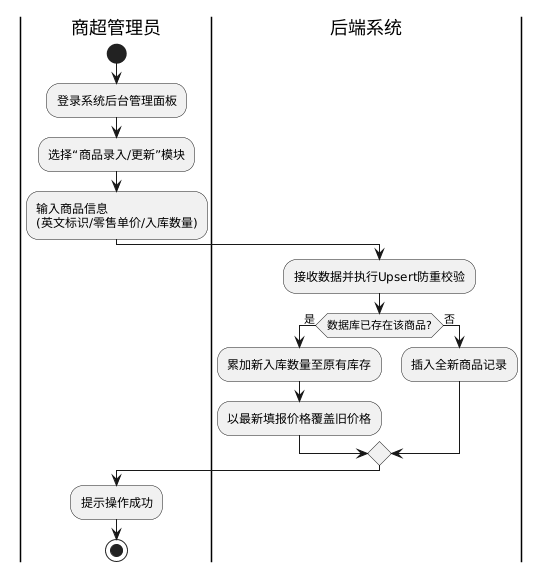
\includegraphics[width=0.88\textwidth]{images/图3-2.png}\\[0.3em]
  {\zihao{-5}图3-2}
\end{center}

\subsection{功能用例分析}

\subsubsection{视觉识别与定位分析（UC-01）}
\begin{itemize}[leftmargin=2em]
  \item 用例名称：视觉识别与物品定位
  \item 用例编号：UC-01
  \item 参与者：顾客
  \item 前置条件：系统后台服务已正常启动；YOLO 模型权重文件已正确加载；操作系统已授予 Python 进程访问本地摄像头的硬件权限。
  \item 主要事件流（Main Flow）：
\end{itemize}
\begin{enumerate}[leftmargin=2.6em]
  \item 顾客浏览系统主界面的货架商品列表，选择目标商品，点击“定位寻物”按钮。
  \item 前端界面锁定该按钮防止重复提交，并通过异步请求（Fetch API）通知后端视觉服务。
  \item 后端视觉处理中心利用 subprocess 模块拉起独立的 YOLO 推理脚本。
  \item 视觉脚本捕捉摄像头实时帧序列，进行图像预处理，喂入 YOLO 模型进行毫秒级目标检测运算。
  \item 模型输出包含分类标签、置信度以及 Bounding Box 坐标（x1, y1, x2, y2）的张量数据。
  \item 系统过滤非目标物品数据，计算目标物品屏幕中心坐标，并在独立的监控窗口上绘制绿色高亮边框与红色中心准星。
  \item 顾客根据屏幕指引在物理货架上准确找到商品。
\end{enumerate}

\begin{itemize}[leftmargin=2em]
  \item 备选事件流（Alternative Flow）：
  \item 物品未找到（A1）：如果在视频流中持续 N 帧未检测到目标类别的置信度 \(\geq\) 预设阈值（如 0.5），则系统在监控窗口上方显示醒目的红色文本提示“未在画面中找到物品”。
  \item 后置条件：顾客完成选购，按 'q' 键释放摄像头资源，系统非阻塞地安全销毁视觉推理子进程。
\end{itemize}

\begin{center}
  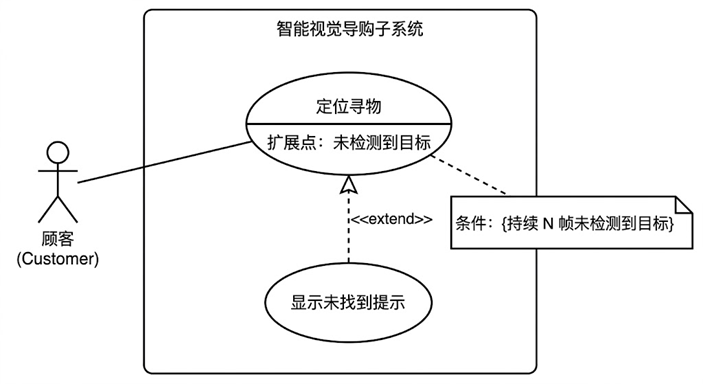
\includegraphics[width=0.88\textwidth]{images/图3-3.png}\\[0.3em]
  {\zihao{-5}图3-3}
\end{center}

\subsubsection{购物车管理与批量结算（UC-03, UC-04）}
\begin{itemize}[leftmargin=2em]
  \item 用例名称：购物车管理与批量结算
  \item 用例编号：UC-03/04（复合用例）
  \item 参与者：顾客
  \item 前置条件：顾客身份已通过登录校验；数据库处于非锁定状态。
  \item 触发条件：顾客完成商品挑选后，主动点击“结算”按钮。
  \item 业务规则：同一商品重复加入购物车时仅累加数量；结算金额统一保留两位小数；结算接口需校验一次性请求标识（Token）以避免重复扣款。
  \item 主要事件流（Main Flow）：
\end{itemize}
\begin{enumerate}[leftmargin=2.6em]
  \item 顾客在系统前端货架列表中点击商品旁的“+ 加入购物车”按钮。
  \item 前端动态更新内存中的购物车对象，实时计算并显示当前金额总计。
  \item 顾客可在购物车面板中增减商品数量、删除单项商品，并实时查看金额变化。
  \item 顾客点击“一键刷脸结算”按钮。
  \item 前端将完整的 JSON 清单请求发送至后端结算 API。
  \item 后端开启数据库事务。遍历清单，锁定 products 表对应行记录，执行原子扣减操作：stock = stock - buy\_quantity。
  \item 计算所有单品的花费金额总计。在 orders 表中为该顾客写入一条全新的销售订单记录。
  \item 后端返回订单摘要（订单 ID、金额、时间戳、购买清单），前端进行成功态渲染。
  \item 提交数据库事务。前端清空本地购物车缓存，向顾客展示模拟扣款成功的回执界面（包含订单 ID、消费金额）。
\end{enumerate}

\begin{itemize}[leftmargin=2em]
  \item 异常事件流（Exception Flow）：
  \item 库存不足（E1）：在遍历结算清单时，系统检测到某单品的现有库存量小于其购买量。后端拦截交易，回滚数据库事务，并向前端返回报错信息：“【商品 A】库存不足，结算失败！”。
  \item 重复提交（E2）：当顾客连续点击结算按钮导致同一 Token 重复到达时，后端仅受理首个请求，其余请求返回“订单已处理”提示，不再进行二次扣减。
  \item 订单写入失败（E3）：若订单写入阶段发生数据库异常，系统执行事务回滚，并提示“系统繁忙，请稍后重试”。
  \item 后置条件：订单状态被持久化存储；前端恢复初始货架状态；系统静默触发库存预警用例（UC-07）。
\end{itemize}

\begin{center}
  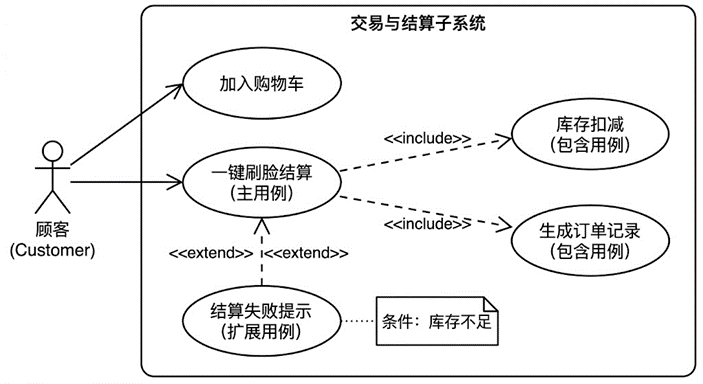
\includegraphics[width=0.88\textwidth]{images/图3-4.png}\\[0.3em]
  {\zihao{-5}图3-4}
\end{center}

\subsubsection{商品信息维护管理（UC-05）}
\begin{itemize}[leftmargin=2em]
  \item 用例名称：商品信息维护管理
  \item 用例编号：UC-05
  \item 参与者：商超管理员
  \item 前置条件：管理员已通过鉴权登录系统后台。
  \item 触发条件：管理员进入“商品维护”页面并提交新增或更新请求。
  \item 业务规则：商品英文标识必须与模型类别名一致；单价必须大于 0；库存数量必须为非负整数。
  \item 主要事件流（Main Flow）：
\end{itemize}
\begin{enumerate}[leftmargin=2.6em]
  \item 管理员进入后台维护面板，输入商品的英文标识名称（需匹配 YOLO 推理脚本分类标签）。
  \item 管理员选择“新品上架”或“库存补录”模式，输入单价和入库数量（例如 50）。
  \item 管理员点击提交。后端拦截该数据。
  \item 后端执行字段合法性校验（名称、价格、库存）。
  \item 系统执行 Upsert 逻辑：先在数据库中检索是否存在同名商品。
  \item 如果存在，则更新价格并将新入库量累加至旧库存（stock = existing\_stock + 50）。
  \item 如果不存在，则创建全新商品记录（INSERT），设置初始库存。
  \item 系统记录本次操作日志（操作者、时间、变更前后值），用于审计追踪。
\end{enumerate}

\begin{itemize}[leftmargin=2em]
  \item 异常事件流（Exception Flow）：
  \item 标签不匹配（E1）：商品名称与模型类别集不一致时，系统拒绝写入并提示“商品标签未在视觉模型中注册”。
  \item 字段非法（E2）：当价格小于等于 0 或库存为负值时，系统返回参数校验失败信息。
  \item 数据库不可用（E3）：写入过程中数据库连接异常，系统返回失败信息并保留原数据。
  \item 后置条件：管理员接收前端“数据维护成功”的提示信息；本地数据库数据已同步更新。
\end{itemize}

\begin{center}
  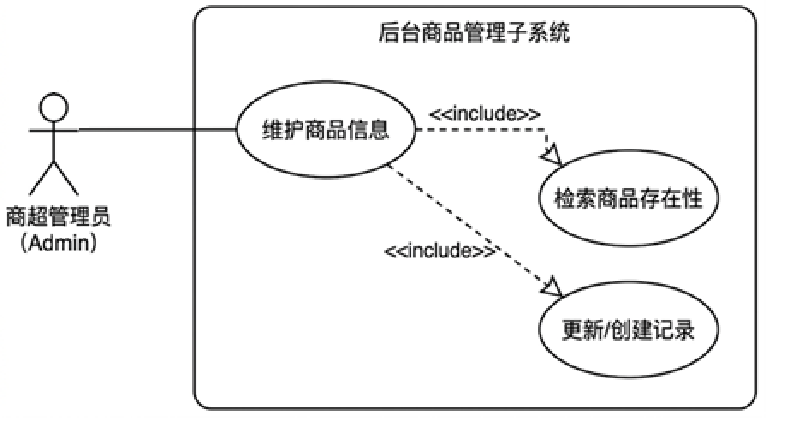
\includegraphics[width=0.88\textwidth]{images/图3-5.png}\\[0.3em]
  {\zihao{-5}图3-5}
\end{center}

\subsubsection{销售数据统计大盘（UC-06）}
\begin{itemize}[leftmargin=2em]
  \item 用例名称：销售数据统计大盘
  \item 用例编号：UC-06
  \item 参与者：商超管理员
  \item 前置条件：系统处于运营状态，数据库中存在历史订单记录。
  \item 触发条件：管理员打开“统计报表”页面或主动点击“刷新报表”。
  \item 业务规则：统计周期默认按自然日聚合；金额统一以人民币元为单位保留两位小数；Top 榜单按销量降序展示。
  \item 主要事件流（Main Flow）：
\end{itemize}
\begin{enumerate}[leftmargin=2.6em]
  \item 管理员进入后台数据报表面板。
  \item 前端自动向后端 API 请求聚合统计数据。
  \item 后端利用 SQL 聚合函数在 orders 表上执行 Group By 操作。计算核心指标：当天总营业额、总单量、总销售件数。计算销售件数 Top 5 畅销商品排行榜。
  \item 系统将计算结果封装为标准 JSON 格式并返回。
  \item 前端利用图表库（如简单的 html/js 表格）将数据进行可视化渲染呈现给管理员。
  \item 管理员可选择导出当天统计快照（CSV）用于离线分析。
\end{enumerate}

\begin{itemize}[leftmargin=2em]
  \item 异常事件流（Exception Flow）：
  \item 无订单数据（E1）：若当前统计周期内无有效订单，系统返回零值统计并提示“暂无销售数据”。
  \item 查询超时（E2）：聚合查询超时则返回缓存数据，并提示“当前展示为最近一次统计快照”。
  \item 可视化渲染失败（E3）：前端图表渲染异常时自动降级为表格文本展示。
  \item 后置条件：统计结果被写入缓存层，供后续页面快速读取。
\end{itemize}

\begin{center}
  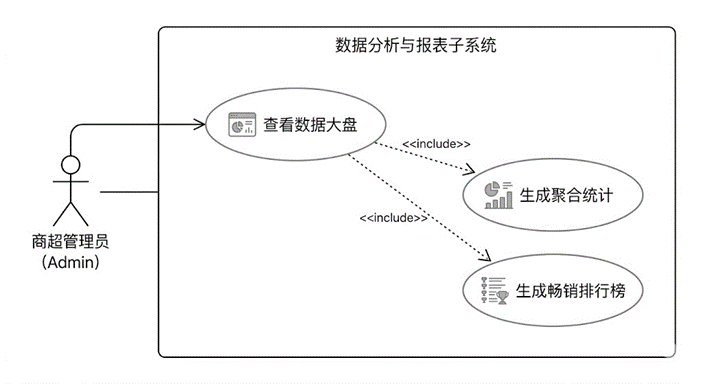
\includegraphics[width=0.88\textwidth]{images/图3-6.png}\\[0.3em]
  {\zihao{-5}图3-6}
\end{center}

\subsubsection{阈值预警与自动补货（UC-07）}
\begin{itemize}[leftmargin=2em]
  \item 用例名称：阈值预警与自动补货
  \item 用例编号：UC-07
  \item 参与者：系统后台（守护进程）、模拟供应商
  \item 前置条件：结算事务（UC-04）成功执行且提交数据库。
  \item 触发条件：订单完成后库存发生变化，触发库存巡检任务。
  \item 业务规则：预警阈值支持按商品维度独立配置；同一商品在同一巡检周期内仅触发一次补货请求；补货默认批量为 50 件。
  \item 主要事件流（Main Flow）：
\end{itemize}
\begin{enumerate}[leftmargin=2.6em]
  \item 系统结算逻辑完成后，触发库存核查钩子（Hook）。
  \item 系统查询刚才被扣减库存的商品（例如 A）在 products 表中最新的剩余库存量。
  \item 系统判断：剩余库存 \(\leq\) 预警阈值（默认=3）？
  \item 如果是，系统后台自动组装标准化补货工单（JSON），包含：请求的外部供应商 API 地址、商品英文名、补货量（例如固定 +50 件）。
  \item 系统将报文 POST 发送至外部模拟供应商的 API 接口。
  \item 接收到供应商返回的发货确认 JSON 回执后，系统在本地数据库强制追加该商品库存（stock = stock + 50），并生成补货系统日志供管理员查阅。
  \item 系统向管理员消息中心推送“自动补货已执行”的通知，附带商品名称与补货数量。
\end{enumerate}

\begin{itemize}[leftmargin=2em]
  \item 异常事件流（Exception Flow）：
  \item 供应商接口不可达（E1）：若外部 API 请求失败，系统将补货任务写入重试队列并按指数退避策略重试。
  \item 供应商回执异常（E2）：当回执字段缺失或状态码非法时，系统不更新库存并标记任务为“人工复核”。
  \item 并发冲突（E3）：当库存记录被其他事务占用时，系统等待短时重试，超过阈值后转入补偿任务队列。
  \item 后置条件：供应链补给流程完成，无需人工干预。
\end{itemize}

\begin{center}
  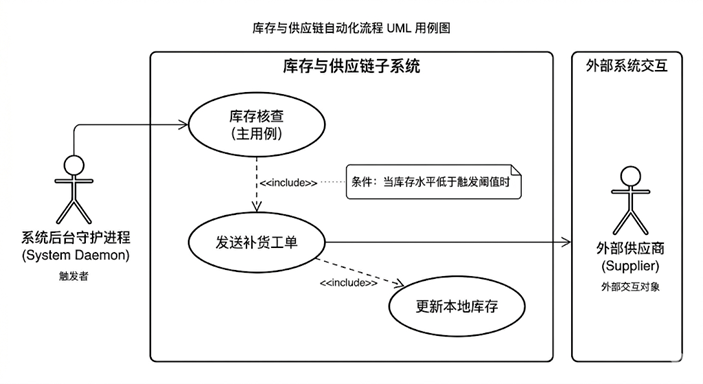
\includegraphics[width=0.88\textwidth]{images/图3-7.png}\\[0.3em]
  {\zihao{-5}图3-7}
\end{center}

\subsection{数据流分析}
本节通过数据流图（DFD）自顶向下地分析系统内外部的数据流转过程，主要包含顶层数据流图和一层数据流图。

\subsubsection{顶层数据流图}
顶层数据流图主要界定了“智能零售系统”的边界，以及它与外部实体（顾客、管理员、供应商）之间的顶层数据交互。

\begin{center}
  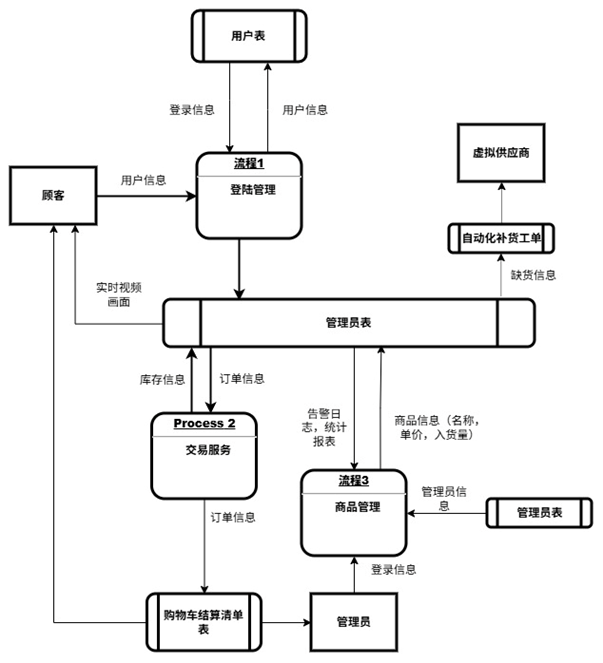
\includegraphics[width=0.88\textwidth]{images/图3-8.png}\\[0.3em]
  {\zihao{-5}图3-8}
\end{center}

\subsubsection{一层数据流图}
一层数据流图主要界定了“智能零售系统”的边界，以及它与外部实体（顾客、管理员、供应商）之间的顶层数据交互。

  \quad
  \quad
\begin{center}
  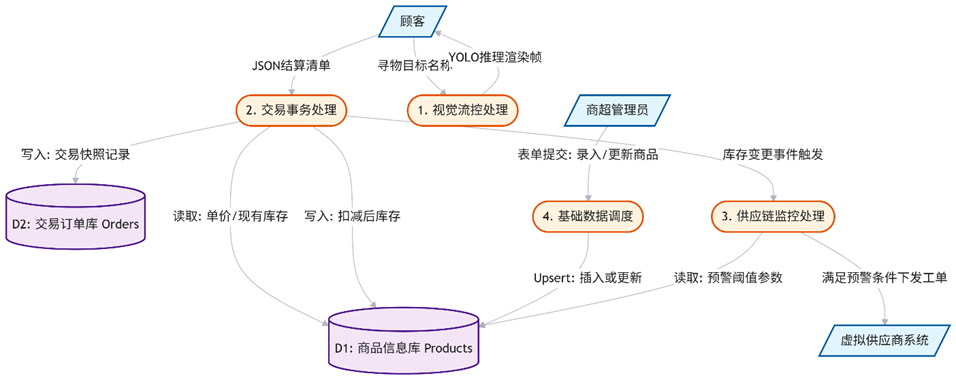
\includegraphics[width=0.88\textwidth]{images/图3-9.png}\\[0.3em]
  {\zihao{-5}图3-9}
\end{center}

\section{非功能性需求}

\subsection{性能需求}
\begin{itemize}[leftmargin=2em]
  \item 算法推理延迟：在配备 NVIDIA GPU 的计算环境下，YOLOv8 模型对单帧图像的推理时间应 \(\leq\) 30ms，保证视频流视觉无明显卡顿（\(>\)25 FPS）。
  \item 接口响应时间：除视觉处理外的所有在线数据 API（如获取商品列表、批量结算），在本地回环网络下的响应时间必须 \(\leq\) 200ms。
  \item 识别准确率：在光照充足、商品无严重遮挡的理想商超环境下，算法对已训练目标的识别召回率（Recall）应达到 90\% 以上。
\end{itemize}

\subsection{安全性需求}
\begin{itemize}[leftmargin=2em]
  \item 并发隔离：视觉推理模块必须与后端 Web 服务器（Uvicorn）在不同进程中运行（通过子进程拉起），防止因摄像头异常或显存溢出导致整个收银系统崩溃。
  \item 数据一致性：结算扣款与库存扣减必须置于同一个数据库事务（Transaction）中处理。若库存不足，必须全部回滚，严禁出现“钱已扣但库存未减”的脏写现象。
  \item 防注入攻击：前后端数据交互严格遵守 RESTful 规范，利用 Pydantic 模型进行强制数据类型校验，防止恶意的 SQL 注入或格式越界。
\end{itemize}

\subsection{易用性需求}
\begin{itemize}[leftmargin=2em]
  \item 极简部署：系统需提供 requirements.txt 或 environment.yml，确保在一台全新计算机上可通过简单的命令实现一键环境复原。
  \item UI 容错机制：前端界面对所有网络请求异常（如后端服务未启动、接口 404）进行捕获，并以弹窗或红色醒目文字的形式给出人类可读的提示（如“网络错误，无法连接后端”），禁止出现控制台级报错直接暴露给普通用户。
\end{itemize}
